\section{Data Requirements}\label{sec:data_requirements}

 An age-based model refers to how \CNAME\ keeps track of the population, which is by keeping track of the numbers-at-age in each year for each category in the population.

The information that is required to set up and run an age-based model in \CNAME\ can be minimal, and can be expanded to include other functionality.

\begin{enumerate}
	\item Time series of catch (currently this is assumed to be known without error)
	\item Time series of relative/absolute abundance/biomass
	\item Age/length composition data (to estimate selectivity ogives or year class strengths)
	\item Information about recruitment and the stock-recruit process
	\item Biological information (e.g., growth, maturity, natural mortality, life cycle)
\end{enumerate}

The minimum amount of information needed to run a \CNAME\ model is recruitment and biological information. Such a model would not include any fishing exploitation processes and so would be an equilibrium or steady-state model.

The biological information that is required depends on whether weight-based calculations will be performed. For an age-based model the parameters for these processes need to be specified:

\begin{enumerate}
	\item length-at-age \command{age\_length}
	\item weight-at-length \command{length\_weight}
	\item natural mortality-at-age \command{selectivity}
\end{enumerate}

\begin{figure}[htp]
			 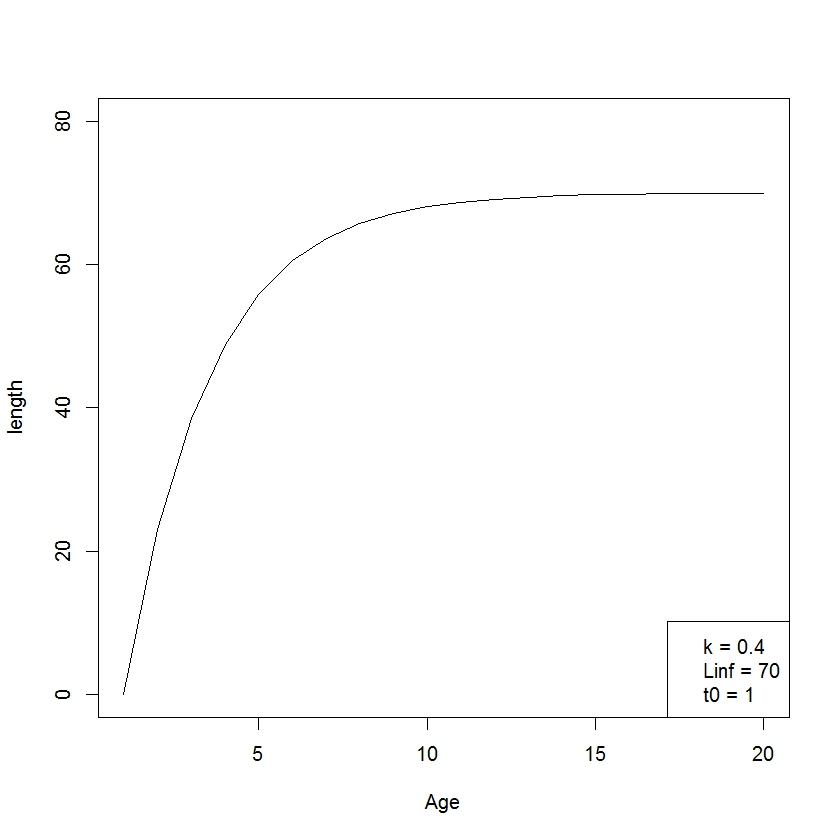
\includegraphics[scale=0.4]{Figures/VonBert.jpeg}
			 \caption{\textbf{An example of a Von Bertalanfy growth curve.}}
\end{figure}



